\documentclass[11pt]{article}

% Language setting
\usepackage[turkish]{babel}
\usepackage{pythonhighlight}

\usepackage[a4paper,top=2cm,bottom=2cm,left=2cm,right=2cm,marginparwidth=2cm]{geometry}

% Useful packages
\usepackage{amsmath}
\usepackage{graphicx}
\usepackage[colorlinks=true, allcolors=blue]{hyperref}
\usepackage{verbatim}
\usepackage{fancyhdr} % for header and footer
\usepackage{titlesec}
\usepackage{parskip}

\setlength{\parindent}{0pt}

\titleformat{\subsection}[runin]{\bfseries}{\thesubsection}{1em}{}

\pagestyle{fancy} % activate the custom header/footer

% define the header/footer contents
\lhead{\small{23BLM-4014 Yapay Sinir Ağları Ara Sınav Soru ve Cevap Kağıdı}}
\rhead{\small{Dr. Ulya Bayram}}
\lfoot{}
\rfoot{}

% remove header/footer on first page
\fancypagestyle{firstpage}{
  \lhead{}
  \rhead{}
  \lfoot{}
  \rfoot{\thepage}
}
 

\title{Çanakkale Onsekiz Mart Üniversitesi, Mühendislik Fakültesi, Bilgisayar Mühendisliği Akademik Dönem 2022-2023\\ 
Ders: BLM-4014 Yapay Sinir Ağları/Bahar Dönemi\\ 
ARA SINAV SORU VE CEVAP KAĞIDI\\
Dersi Veren Öğretim Elemanı: Dr. Öğretim Üyesi Ulya Bayram}
\author{%
\begin{minipage}{\textwidth}
\raggedright
Öğrenci Adı Soyadı: HATİCE SAİKE\\ % Adınızı soyadınızı ve öğrenci numaranızı noktaların yerine yazın
Öğrenci No: 180401042
\end{minipage}%
}

\date{14 Nisan 2023}

\begin{document}
\maketitle

\vspace{-.5in}
\section*{Açıklamalar:}
\begin{itemize}
    \item Vizeyi çözüp, üzerinde aynı sorular, sizin cevaplar ve sonuçlar olan versiyonunu bu formatta PDF olarak, Teams üzerinden açtığım assignment kısmına yüklemeniz gerekiyor. Bu bahsi geçen PDF'i oluşturmak için LaTeX kullandıysanız, tex dosyasının da yer aldığı Github linkini de ödevin en başına (aşağı url olarak) eklerseniz bonus 5 Puan! (Tavsiye: Overleaf)
    \item Çözümlerde ya da çözümlerin kontrolünü yapmada internetten faydalanmak, ChatGPT gibi servisleri kullanmak serbest. Fakat, herkesin çözümü kendi emeğinden oluşmak zorunda. Çözümlerinizi, cevaplarınızı aşağıda belirttiğim tarih ve saate kadar kimseyle paylaşmayınız. 
    \item Kopyayı önlemek için Github repository'lerinizin hiçbirini \textbf{14 Nisan 2023, saat 15:00'a kadar halka açık (public) yapmayınız!} (Assignment son yükleme saati 13:00 ama internet bağlantısı sorunları olabilir diye en fazla ekstra 2 saat daha vaktiniz var. \textbf{Fakat 13:00 - 15:00 arası yüklemelerden -5 puan!}
    \item Ek puan almak için sağlayacağınız tüm Github repository'lerini \textbf{en geç 15 Nisan 2023 15:00'da halka açık (public) yapmış olun linklerden puan alabilmek için!}
    \item \textbf{14 Nisan 2023, saat 15:00'dan sonra gönderilen vizeler değerlendirilmeye alınmayacak, vize notu olarak 0 (sıfır) verilecektir!} Son anda internet bağlantısı gibi sebeplerden sıfır almayı önlemek için assignment kısmından ara ara çözümlerinizi yükleyebilirsiniz yedekleme için. Verilen son tarih/saatte (14 Nisan 2023, saat 15:00) sistemdeki en son yüklü PDF geçerli olacak.
    \item Çözümlerin ve kodların size ait ve özgün olup olmadığını kontrol eden bir algoritma kullanılacaktır. Kopya çektiği belirlenen vizeler otomatikman 0 (sıfır) alacaktır. Bu nedenle çözümlerinizi ve kodlarınızı yukarıda sağladığım gün ve saatlere kadar kimseyle paylaşmayınız.
    \item Bu vizeden alınabilecek en yüksek not 100'dür. Toplam aldığınız puan 100'ü geçerse, aldığınız not 100'e sabitlenecektir.
    \item LaTeX kullanarak PDF oluşturanlar öz geçmişlerine LaTeX bildiklerini de eklemeyi unutmasınlar :)
    \item Bu vizedeki soruların çözümleri ve tex dosyası için istediğiniz kadar sayıda Github repository'si oluşturabilirsiniz. Sadece yukarıda belirttiğim tarihlerde (14 Nisan 2023 saat 15:00 ile 15 Nisan 2023 saat 15:00 arasında) public yapmayı/halka açmayı ve Github profilinizi de öz geçmişinize eklemeyi unutmayın :)
    \item Bilgisayarınıza hiçbir program kurmadan, Overleaf, Google Colab, Kaggle gibi ortamlar üzerinden bu vizeyi tamamlamanız mümkün. İyi çalışmalar!!
\end{itemize}

(Ekstra 5 puan) \url{https://github.com/haticesaike/neural_network_mid/blob/main/neural.tex}

\newpage
\section{(Toplam 10 Puan) Hopfield Networks:}

\subsection{(2 Puan)} \textbf{ChatGPT’ye size Hopfield Network’ler ile ilgili detaylı bilgi vermesini isteyin. Sorduğunuz soruyu, ChatGPT'nin çıkartığı cevabı aşağı koyun. Bu cevapta anlamadığınız terimleri de ChatGPT’ye sorup, sorduğunuz soruları ve ChatGPT’nin verdiği cevapları da sırayla aşağı koyun.}

\textbf{SORU:} Hopfield Network’leri nedir, hangi amaçla, nerede kullanılır? Hangi problemi çözer ve nasıl kullanılır, detaylı açıklayabilir misin?

\textbf{CEVAP:} Tabii, size yardımcı olmaktan mutluluk duyarım.

Hopfield ağları, yapay sinir ağı türlerinden biridir ve özellikle bellek işlevlerini simüle etmek için kullanılır. Bu ağlar, içindeki düğümlerin birbirleriyle bağlantıları aracılığıyla bilgi depolama ve hatırlama işlevlerini yerine getirirler.

Hopfield ağları, özellikle optimizasyon problemlerini çözmek için tasarlanmıştır. Optimizasyon problemleri, bir fonksiyonun minimum veya maksimum değerini bulma gibi matematiksel veya mühendislik problemleridir. Hopfield ağları, enerji fonksiyonları kullanarak bu optimizasyon problemlerini çözmek için kullanılır. Ağ, enerji fonksiyonunu minimize etmek için girdi verileri üzerinde çalışır.

Bir Hopfield ağı, bir matris şeklinde ifade edilebilir. Bu matris, ağın düğümleri arasındaki bağlantıları gösterir. Matrisin köşegenleri sıfırdır, çünkü bir düğüm kendisiyle doğrudan bağlantılı değildir. Ağın diğer bağlantıları simetrik olmalıdır, çünkü bağlantılar birbirine bağımlıdır.

Hopfield ağları, verilerin depolanması, tanınması ve sıkıştırılması gibi birçok alanda kullanılır. Örneğin, Hopfield ağına bir dizi resim verilebilir ve ağ, benzer özelliklere sahip resimleri gruplayarak verileri sıkıştırabilir. Ayrıca, Hopfield ağı, ham verileri temizleyebilir veya eksik verileri tamamlayabilir.

Hopfield ağları, yapay sinir ağlarına giriş yapmak isteyenler için de bir başlangıç noktası olarak kullanılabilir. Bu ağlar, basit yapısı ve kolayca anlaşılabilirliği sayesinde yapay sinir ağları hakkında genel bir anlayış sağlamak için kullanılabilirler.

Hopfield ağlarının kullanımı, ağın nasıl eğitildiğine bağlıdır. Bir Hopfield ağı, ağın girdilerinin hepsinin aynı anda verilmesiyle eğitilir. Eğitim işlemi sırasında, ağ girdi verilerini depolar ve enerji fonksiyonunu minimize etmek için çalışır. Eğitim tamamlandığında, ağ verilen bir girdiye en yakın olan depolanan veriyi hatırlayabilir veya verileri sıkıştırabilir.

\textbf{Bellek işlevlerini simüle etmek derken neyi kastediyorsun açıklar mısın?}

Hopfield ağları, insan belleği gibi bilgi depolama ve hatırlama işlevlerini simüle etmek için kullanılır. Bu ağlar, öğrenme yoluyla veri örüntülerini depolayabilir ve daha sonra bu örüntüleri hatırlamak için kullanabilir. Ayrıca, veri örüntüleri arasındaki benzerlikleri tanıyabilir ve sınıflandırabilirler.

Hopfield ağları, birçok alanda bellek işlevlerini simüle etmek için kullanılabilir. Örneğin, birçok uygulama, Hopfield ağlarını görüntülerin tanınması, yüz tanıma, ses tanıma, doğal dil işleme ve finansal tahminler gibi alanlarda kullanır.

Özetle, Hopfield ağları, bellek işlevlerini simüle ederek, bir veri kümesindeki örüntüleri depolayabilir ve daha sonra bu örüntüleri hatırlayabilirler. Bu, birçok uygulamada kullanılabilen güçlü bir özelliktir.

\textbf{Hopfield ağlarının çözdüğü optimizasyon problemlerine bir örnek verir misin?}

Tabii, bir örnek vermek gerekirse, Hopfield ağları, seyahat eden satıcı problemi gibi NP-zorlu optimizasyon problemlerini çözmek için kullanılabilir. Seyahat eden satıcı problemi, bir satıcının verilen bir dizi şehre en kısa yolculuk mesafesiyle gitmesi gereken bir problem olarak tanımlanabilir. Bu problem, sayısal yöntemlerle çözülebilir ancak Hopfield ağları gibi alternatif yaklaşımlar da kullanılabilir. Hopfield ağları, seyahat eden satıcı problemi gibi problemleri enerji fonksiyonlarına dönüştürerek çözebilir. Problemin optimal çözümü, enerji fonksiyonunun minimum değerine karşılık gelir. Hopfield ağı, enerji fonksiyonunu minimize ederek optimal çözümü elde eder.


\subsection{(8 Puan)} \textbf{ChatGPT’nin açıklamalarından ne anladığınızı buraya kendi kelimelerinizle özetleyin. Örneğin ``Hopfield Network nedir? Ne işe yarar? Neden bilmemiz gerekir bunu? Gerçek hayatta kullanılıyor mu?'' gibi. Anlamadığınız kısımlar varsa ve ChatGPT’nin açıklamaları yeterli gelmezse internet dahil farklı kaynaklardan araştırıp, bilgilerin doğruluğunu sorgulamakta serbestsiniz. Konuyu doğru anlayıp anlamamanız puana etki edecektir. Kullandığınız kaynakları da belirtin!}

Hopfield ağları, yapay sinir ağı olarak isimlendirilir. İnsan zihnindeki bilgiler sinir ağları aracılığı ile iletilir ve yine aynı ağ aracılığı ile çeşitli bilgileri analiz edip, harmanlayarak bir cevap döndürür. Hopfield ağları insan zihninin bu işleyişinin simüle edilmiş hali gibi düşünülebilir. Hopfield ağları kendi içinde bi sürü bilgi ağı oluşturur ve bu ağların içindeki verileri bağlantılı olduğu diğer verileri de baz alarak yorumlar, böylece bir karar mekanizması oluşmuş olur. Birtakım bilgileri temel almasını söyleyerek yeni bilgileri önceki veriler ışığında yorumlamasını sağlıyoruz aslında. Örneğin eğitilmiş bir dataset verdiğimizi varsayalım, içinde people labelına sahip resimler yer alsın. Hopfield ağlarının da  sayesinde bu bilgiler depolanır ve benzer bir resim gördüğünde people olup olmadığıyla ilgili yorum yapabilecek bir mekanizmaya sahip olur. Yani Hopfield ağları, birtakım verileri depolama, analiz etme ve gerektiğinde kullanabilmeyi sağlayan bir bilgi ağıdır, diyebiliriz. Kullanım alanı geniş olmakla beraber özellikle makine öğrenmesi konusunda hopfield ağlarından yararlanılabileceğini düşünüyorum .Ayrıca yüz tanıma, ses tanıma gibi programları incelediğimizde hopfield ağlarının gerçek hayatta oldukça etkin bir biçimde kullanıldığını görürüz

\section{(Toplam 10 Puan) Boltzman Machine:}

\subsection{(2 Puan)} \textbf{ChatGPT’ye size Boltzman Machine ilgili detaylı bilgi vermesini isteyin. Sorduğunuz soruyu, ChatGPT'nin çıkartığı cevabı aşağı koyun. Bu cevapta anlamadığınız terimleri de ChatGPT’ye sorup, sorduğunuz soruları ve ChatGPT’nin verdiği cevapları da sırayla aşağı koyun.}

\textbf{SORU:} Boltzman Machine nedir, ne işe yarar, hangi ihtiyaçtan doğmuştur detaylı bir şekilde açıklayabilir misin?

\textbf{CEVAP:} Bir Boltzmann makinesi, yapay sinir ağı alanında bir tür denetimsiz öğrenme algoritmasıdır. Adını, istatistik mekaniği ve termodinamiği alanında çalışmalar yapmış olan Ludwig Boltzmann'dan almaktadır. Boltzmann makinesi, hem girdi hem de çıktı katmanına sahip olan bir yapay sinir ağıdır ve unsupervised learning (denetimsiz öğrenme) için tasarlanmıştır.

Bir Boltzmann makinesi, iki tür düğümden oluşur: gizli düğümler ve görünür düğümler. Gizli düğümler, ağın içinde bulunurlar ve diğer düğümlere bağlıdırlar. Görünür düğümler ise ağın girdi katmanını oluşturur ve dışarıdan verilen verileri temsil ederler. Bu veriler, ağın gizli düğümleri tarafından işlenir ve sonuç olarak ağın çıktıları elde edilir.

Boltzmann makinesi, belirli bir veri setini öğrenmek için kullanılır. Bu veri seti, ağın girdi katmanına verilir ve ağın gizli düğümleri, verilerin belirli özelliklerini öğrenmek için birbirleriyle etkileşime girerler. Bu özellikler, ağın öğrenme sürecinde otomatik olarak belirlenir ve veri setinin genel yapısını temsil eder.

Boltzmann makinesi, birçok alanda kullanılır. Özellikle, verilerin boyutunu azaltmak veya gizli yapıları ortaya çıkarmak için kullanılır. Örneğin, bir görüntü veri setindeki yüzleri tanımak için kullanılabilir. Ayrıca, doğal dil işleme ve sınıflandırma gibi diğer alanlarda da kullanılabilir.

Boltzmann makinesi, öğrenme sırasında enerji fonksiyonu olarak adlandırılan bir fonksiyonu minimize etmek için çalışır. Bu enerji fonksiyonu, ağın girdi verilerini ve ağın gizli düğümlerini kullanarak hesaplanır. Ağın öğrenme işlemi, enerji fonksiyonunun minimum değerini bulmak için gerçekleştirilir. Bu minimum değer, ağın verileri en iyi şekilde temsil edebilecek bir konfigürasyona sahip olduğunu gösterir.

Boltzmann makinesinin tasarlanması, yapay sinir ağlarının denetimsiz öğrenme ihtiyacından doğmuştur. Denetimsiz öğrenme, özellikle büyük veri setleri üzerinde çalışırken verilerin birçoğunun etiketlenmemesi durumunda kullanışlıdır.

\textbf{Unsupervised learning nedir?}

Unsupervised learning, makine öğrenmesi alanında, etiketlenmemiş verilerin kullanılarak yapılan öğrenme yöntemidir. Bu yöntemde, veri kümesindeki herhangi bir özellik veya sınıflandırma bilgisi verilmez ve model kendi kendine verilerdeki yapıları keşfetmeye çalışır.

Unsupervised learning, verilerin özelliklerini ve desenlerini keşfetmek için kullanılabilir. Bu, veri setindeki benzer özelliklere sahip örnekleri gruplandırma, benzer olmayan özellikleri olan örnekleri ayırma ve verilerin boyutunu azaltma gibi işlemleri içerebilir.

Bu yöntem, geniş veri setlerinde veri keşfi ve ön işleme için sıklıkla kullanılır. Ayrıca, kümeler arasındaki ilişkileri belirlemek veya verilerin gizli yapılarını öğrenmek için kullanılabilir.

Örnek olarak, bir restoranın müşterilerinden gelen sipariş verilerini ele alabiliriz. Sipariş verilerindeki herhangi bir sınıflandırma bilgisi olmadan, unsupervised learning yöntemleri kullanarak benzer ürünleri bir araya getirebilir ve bu bilgiyi restoranın menüsünde kullanabiliriz. Bu sayede müşterilerin ilgi alanlarını daha iyi anlayabilir ve onlara daha iyi bir deneyim sunabiliriz.

\subsection{(8 Puan)} \textbf{ChatGPT’nin açıklamalarından ne anladığınızı buraya kendi kelimelerinizle özetleyin. Örneğin ``Boltzman Machine nedir? Ne işe yarar? Neden bilmemiz gerekir bunu? Gerçek hayatta kullanılıyor mu?'' gibi. Anlamadığınız kısımlar varsa ve ChatGPT’nin açıklamaları yeterli gelmezse internet dahil farklı kaynaklardan araştırıp, bilgilerin doğruluğunu sorgulamakta serbestsiniz. Konuyu doğru anlayıp anlamamanız puana etki edecektir. Kullandığınız kaynakları da belirtin!}

Boltzman makinesi bir denetimsiz öğrenme algoritmasıdır. Gizli ve görünür düğümlerden oluşur.Görünür düğümler dışarıdan girilen verilerdir. Gizli düğümler görünür düğümlerden gelen bilgileri işleyerek bir çıktı oluşturur. Belirli bir dataseti öğrenmek için kullanılabilir.Dataset girdi katmanı olarak verilir ve gizli katman, girdi katmanında yer alan datasetin verilerini kullanarak belirli özellikleri öğrenmeye çalışır.Ancak datasetteki veriler etiketli değildir,denetimsiz öğrenme derken kastedilen de budur. Gizli katmanda belirli özeliklerden ortak paydalar çıkarılır ve veriler bu kümeleme sonucunda kategorize edilir. Boltzman makinesinde kullanılan ve analizin başarısını tespit etmeye yarayan enerji fonksiyonu vardır. Bu fonksiyonun değeri ne kadar küçük çıkarsa öğrenme o kadar başarılı sayılır. Süreç boyunca amaç enerji fonksiyonunu minimum düzeye çekmektir.

\section{(Toplam 10 Puan) Markov Assumption ve Markov Chain:}

\subsection{(2 Puan)} \textbf{ChatGPT’ye size Markov assumption ve Markov Chain ilgili detaylı bilgi vermesini isteyin. Sorduğunuz soruyu, ChatGPT'nin çıkartığı cevabı aşağı koyun. Bu cevapta anlamadığınız terimleri de ChatGPT’ye sorup, sorduğunuz soruları ve ChatGPT’nin verdiği cevapları da sırayla aşağı koyun.}

\textbf{SORU:}  Markov assumption ve Markov Chain nedir, nerede kullanılır detaylı açıklar mısın?

\textbf{CEVAP:} Markov assumption, bir durumun gelecekteki davranışının yalnızca mevcut duruma bağlı olduğunu varsayar. Yani, bir sistemin gelecekteki davranışı, sadece şu anki durumuna bağlıdır ve geçmiş durumları veya olayları dikkate almaz. Bu varsayım, Markov Chain (Markov Zinciri) olarak adlandırılan bir olasılık modeli için temel bir varsayımdır.

Markov Chain, bir dizi durumun ardışık olarak oluştuğu ve her durumun yalnızca mevcut duruma bağlı olduğu bir olasılık sürecidir. Bu durumlar birbirine bağlıdır ve her bir durumun gerçekleşme olasılığı, yalnızca önceki durumun gerçekleşme olasılığına bağlıdır. Yani, Markov Chain'de, bir durumun gerçekleşme olasılığı, yalnızca önceki durumun gerçekleşme olasılığına bağlıdır ve diğer geçmiş durumlar veya olaylar göz önüne alınmaz.

Markov Chain, birçok alanda kullanılır. Örneğin, doğal dil işleme (NLP) ve makine çevirisi alanlarında sıklıkla kullanılır. Burada, bir kelimenin veya kelime dizisinin önceki kelimelere bağlı olarak olasılığı modellenir. Finansal piyasalar ve ekonomi gibi alanlarda da kullanılır. Burada, fiyat hareketlerinin ardışık durumları modellenir ve gelecekteki fiyatların tahmin edilmesine yardımcı olur. Ayrıca, zaman serileri analizi, rastgele yürüyüş modelleri, sinyal işleme ve kontrol sistemleri de Markov Chain kullanım alanlarıdır.

Markov Chain, özellikle belirli koşullar altında, istatistiksel olarak tahmin edilebilir bir yapıya sahiptir. Bu nedenle, Markov Chain, belirli bir sürecin öngörülebilirliğini ve modellenmesini sağlar. Bununla birlikte, Markov Chain'nin uygulanması için sistemin Markov assumption'a uygun olması gerekir, yani gelecekteki durumun yalnızca mevcut duruma bağlı olduğu varsayımı geçerli olmalıdır.

\subsection{(8 Puan)} \textbf{ChatGPT’nin açıklamalarından ne anladığınızı buraya kendi kelimelerinizle özetleyin. Örneğin ``Markov assumption ve Markov Chain nedir? Ne işe yarar? Neden bilmemiz gerekir bunu? Gerçek hayatta kullanılıyor mu?'' gibi. Anlamadığınız kısımlar varsa ve ChatGPT’nin açıklamaları yeterli gelmezse internet dahil farklı kaynaklardan araştırıp, bilgilerin doğruluğunu sorgulamakta serbestsiniz. Konuyu doğru anlayıp anlamamanız puana etki edecektir. Kullandığınız kaynakları da belirtin!}

Markov assumption, gelecekteki bir durumun gerçekleşme olasılığının  sadece bugünkü durum bilgisine bağlı olduğunu varsayar. Yani bir durumla ilgili olasılıklar geçmişteki durumlardan bağımsızdır, sadece bugünkü durum bilgisi önemlidir. Markov Chain ise Markov assumption'u temel alan bir matematiksel olasılık modelidir. Markov Chain'nin uygulanması için gelecekteki durumun yalnızca mevcut duruma bağlı olduğu varsayımı geçerli olmalıdır. Markov Chain'e göre birbirine bağlı olan olasılık durumlarından herbirinin gerçekleşme olasılığı sadece önceki durumun gerçekleşme olasılığınıa bağlıdır. Bu model birçok alanda kullanılır, örneğin makine çevirisi alanında bi kelime veya kelime grubunun önceki kelimelere bağlı olarak ne olabileceği tahmin edilir.Benzer mantıkla hava durumu tahmininde de kullanılır. Bir hava durumu tahmini yapmak için, bugünkü hava durumunu "durum" olarak kabul edilebilir. Daha sonra, geçiş olasılıkları, bugünkü durumun yarınki duruma geçiş olasılığını gösterir. Yani geçmişteki hava durumlarından bağımsız havanın bugünkü durumuna göre gelecekte olabilecek durumlar için olasılıklar oluşturulur.

\section{(Toplam 20 Puan) Feed Forward:}
 
\begin{itemize}
    \item Forward propagation için, input olarak şu X matrisini verin (tensöre çevirmeyi unutmayın):\\
    $X = \begin{bmatrix}
        1 & 2 & 3\\
        4 & 5 & 6
        \end{bmatrix}$
    Satırlar veriler (sample'lar), kolonlar öznitelikler (feature'lar).
    \item Bir adet hidden layer olsun ve içinde tanh aktivasyon fonksiyonu olsun
    \item Hidden layer'da 50 nöron olsun
    \item Bir adet output layer olsun, tek nöronu olsun ve içinde sigmoid aktivasyon fonksiyonu olsun
\end{itemize}

Tanh fonksiyonu:\\
$f(x) = \frac{exp(x) - exp(-x)}{exp(x) + exp(-x)}$
\vspace{.2in}

Sigmoid fonksiyonu:\\
$f(x) = \frac{1}{1 + exp(-x)}$

\vspace{.2in}
 \textbf{Pytorch kütüphanesi ile, ama kütüphanenin hazır aktivasyon fonksiyonlarını kullanmadan, formülünü verdiğim iki aktivasyon fonksiyonunun kodunu ikinci haftada yaptığımız gibi kendiniz yazarak bu yapay sinir ağını oluşturun ve aşağıdaki üç soruya cevap verin.}
 
\subsection{(10 Puan)} \textbf{Yukarıdaki yapay sinir ağını çalıştırmadan önce pytorch için Seed değerini 1 olarak set edin, kodu aşağıdaki kod bloğuna ve altına da sonucu yapıştırın:}

% Latex'de kod koyabilirsiniz python formatında. Aşağıdaki örnekleri silip içine kendi kodunuzu koyun
\begin{python}
import torch
torch.manual_seed(1)
import torch.nn as nn

class Simplenet(nn.Module):
    def __init__(self, input_size=3, hidden_size=50):
        super(Simplenet, self).__init__()
        self.hidden_layer = nn.Sequential(
            nn.Linear(input_size, hidden_size),
            
        )
        self.output_layer = nn.Sequential(
            nn.Linear(hidden_size, 1),
            
        )
    def my_tanh(self,x):
      return (torch.exp(x)-torch.exp(-x))/(torch.exp(x)+torch.exp(-x))

    def my_sigmoid(self,x):
      return 1/ (1+ torch.exp(-x))    
    def forward(self, x):
        x = self.hidden_layer(x)
        x = self.my_tanh(x)
        x = self.output_layer(x)
        x = self.my_sigmoid(x)
        return x

X = torch.tensor([[1, 2, 3], [4, 5, 6]], dtype=torch.float32)
model = Simplenet()
output=model(X)
print(output.data)
\end{python}

tensor([[0.4892],
        [0.5566]])

\subsection{(5 Puan)} \textbf{Yukarıdaki yapay sinir ağını çalıştırmadan önce Seed değerini öğrenci numaranız olarak değiştirip, kodu aşağıdaki kod bloğuna ve altına da sonucu yapıştırın:}

\begin{python}
import torch
torch.manual_seed(180401042)
import torch.nn as nn

class Simplenet(nn.Module):
    def __init__(self, input_size=3, hidden_size=50):
        super(Simplenet, self).__init__()
        self.hidden_layer = nn.Sequential(
            nn.Linear(input_size, hidden_size),
            
        )
        self.output_layer = nn.Sequential(
            nn.Linear(hidden_size, 1),
            
        )
    def my_tanh(self,x):
      return (torch.exp(x)-torch.exp(-x))/(torch.exp(x)+torch.exp(-x))

    def my_sigmoid(self,x):
      return 1/ (1+ torch.exp(-x))    
    def forward(self, x):
        x = self.hidden_layer(x)
        x = self.my_tanh(x)
        x = self.output_layer(x)
        x = self.my_sigmoid(x)
        return x

X = torch.tensor([[1, 2, 3], [4, 5, 6]], dtype=torch.float32)
model = Simplenet()
output=model(X)
print(output.data)
\end{python}

tensor([[0.4695],
        [0.4501]])

\subsection{(5 Puan)} \textbf{Kodlarınızın ve sonuçlarınızın olduğu jupyter notebook'un Github repository'sindeki linkini aşağıdaki url kısmının içine yapıştırın. İlk sayfada belirttiğim gün ve saate kadar halka açık (public) olmasın:}
% size ait Github olmak zorunda, bu vize için ayrı bir github repository'si açıp notebook'u onun içine koyun. Kendine ait olmayıp da arkadaşının notebook'unun linkini paylaşanlar 0 alacak.

\url{https://github.com/haticesaike/neural_network_mid/blob/main/4/Feed_Forward.ipynb}

\section{(Toplam 40 Puan) Multilayer Perceptron (MLP):} 
\textbf{Bu bölümdeki sorularda benim vize ile beraber paylaştığım Prensesi İyileştir (Cure The Princess) Veri Seti parçaları kullanılacak. Hikaye şöyle (soruyu çözmek için hikaye kısmını okumak zorunda değilsiniz):} 

``Bir zamanlar, çok uzaklarda bir ülkede, ağır bir hastalığa yakalanmış bir prenses yaşarmış. Ülkenin kralı ve kraliçesi onu iyileştirmek için ellerinden gelen her şeyi yapmışlar, ancak denedikleri hiçbir çare işe yaramamış.

Yerel bir grup köylü, herhangi bir hastalığı iyileştirmek için gücü olduğu söylenen bir dizi sihirli malzemeden bahsederek kral ve kraliçeye yaklaşmış. Ancak, köylüler kral ile kraliçeyi, bu malzemelerin etkilerinin patlayıcı olabileceği ve son zamanlarda yaşanan kuraklıklar nedeniyle bu malzemelerden sadece birkaçının herhangi bir zamanda bulunabileceği konusunda uyarmışlar. Ayrıca, sadece deneyimli bir simyacı bu özelliklere sahip patlayıcı ve az bulunan malzemelerin belirli bir kombinasyonunun prensesi iyileştireceğini belirleyebilecekmiş.

Kral ve kraliçe kızlarını kurtarmak için umutsuzlar, bu yüzden ülkedeki en iyi simyacıyı bulmak için yola çıkmışlar. Dağları tepeleri aşmışlar ve nihayet "Yapay Sinir Ağları Uzmanı" olarak bilinen yeni bir sihirli sanatın ustası olarak ün yapmış bir simyacı bulmuşlar.

Simyacı önce köylülerin iddialarını ve her bir malzemenin alınan miktarlarını, ayrıca iyileşmeye yol açıp açmadığını incelemiş. Simyacı biliyormuş ki bu prensesi iyileştirmek için tek bir şansı varmış ve bunu doğru yapmak zorundaymış. (Original source: \url{https://www.kaggle.com/datasets/unmoved/cure-the-princess})

(Buradan itibaren ChatGPT ve Dr. Ulya Bayram'a ait hikayenin devamı)

Simyacı, büyülü bileşenlerin farklı kombinasyonlarını analiz etmek ve denemek için günler harcamış. Sonunda birkaç denemenin ardından prensesi iyileştirecek çeşitli karışım kombinasyonları bulmuş ve bunları bir veri setinde toplamış. Daha sonra bu veri setini eğitim, validasyon ve test setleri olarak üç parçaya ayırmış ve bunun üzerinde bir yapay sinir ağı eğiterek kendi yöntemi ile prensesi iyileştirme ihtimalini hesaplamış ve ikna olunca kral ve kraliçeye haber vermiş. Heyecanlı ve umutlu olan kral ve kraliçe, simyacının prensese hazırladığı ilacı vermesine izin vermiş ve ilaç işe yaramış ve prenses hastalığından kurtulmuş.

Kral ve kraliçe, kızlarının hayatını kurtardığı için simyacıya krallıkta kalması ve çalışmalarına devam etmesi için büyük bir araştırma bütçesi ve çok sayıda GPU'su olan bir server vermiş. İyileşen prenses de kendisini iyileştiren yöntemleri öğrenmeye merak salıp, krallıktaki üniversitenin bilgisayar mühendisliği bölümüne girmiş ve mezun olur olmaz da simyacının yanında, onun araştırma grubunda çalışmaya başlamış. Uzun yıllar birlikte krallıktaki insanlara, hayvanlara ve doğaya faydalı olacak yazılımlar geliştirmişler, ve simyacı emekli olduğunda prenses hem araştırma grubunun hem de krallığın lideri olarak hayatına devam etmiş.

Prenses, kendisini iyileştiren veri setini de, gelecekte onların izinden gidecek bilgisayar mühendisi prensler ve prensesler başkalarına faydalı olabilecek yapay sinir ağları oluşturmayı öğrensinler diye halka açmış ve sınavlarda kullanılmasını salık vermiş.''

\textbf{İki hidden layer'lı bir Multilayer Perceptron (MLP) oluşturun beşinci ve altıncı haftalarda yaptığımız gibi. Hazır aktivasyon fonksiyonlarını kullanmak serbest. İlk hidden layer'da 100, ikinci hidden layer'da 50 nöron olsun. Hidden layer'larda ReLU, output layer'da sigmoid aktivasyonu olsun.}

\textbf{Output layer'da kaç nöron olacağını veri setinden bakıp bulacaksınız. Elbette bu veriye uygun Cross Entropy loss yöntemini uygulayacaksınız. Optimizasyon için Stochastic Gradient Descent yeterli. Epoch sayınızı ve learning rate'i validasyon seti üzerinde denemeler yaparak (loss'lara overfit var mı diye bakarak) kendiniz belirleyeceksiniz. Batch size'ı 16 seçebilirsiniz.}

\subsection{(10 Puan)} \textbf{Bu MLP'nin pytorch ile yazılmış class'ının kodunu aşağı kod bloğuna yapıştırın:}

\begin{python}
class MLP(nn.Module):
    def __init__(self):
        super(MLP, self).__init__()
        self.fc1 = nn.Linear(13, 100)
        self.fc2 = nn.Linear(100, 50)
        self.fc3 = nn.Linear(50, 2)
        self.relu = nn.ReLU()
        self.sigmoid = nn.Sigmoid()

    def forward(self, x):
      out = self.fc1(x)
      out = self.relu(out)
      out = self.fc2(out)
      out = self.relu(out)
      out = self.fc3(out)
      out = self.sigmoid(out)
      return out


device = torch.device('cuda' if torch.cuda.is_available() else 'cpu')
model = MLP().to(device)


\end{python}

\subsection{(10 Puan)} \textbf{SEED=öğrenci numaranız set ettikten sonra altıncı haftada yazdığımız gibi training batch'lerinden eğitim loss'ları, validation batch'lerinden validasyon loss değerlerini hesaplayan kodu aşağıdaki kod bloğuna yapıştırın ve çıkan figürü de alta ekleyin.}

\begin{python}
def train(model, optimizer, criterion, train_loader, val_loader, num_epochs):

    best_loss = float('inf')
    for epoch in range(num_epochs):
        running_loss = 0.0
        running_corrects = 0
        total_train = 0
        
        model.train() 
        
        for inputs, labels in train_loader:
            inputs, labels = inputs.to(device), labels.to(device)
            optimizer.zero_grad() 
            
            # forward + backward + optimize
            outputs = model(inputs)
            loss = criterion(outputs, labels)
            
          
            
            loss.backward()
            optimizer.step()
            
            running_loss += loss.item()
            _, preds = torch.max(outputs, 1)
            running_corrects += torch.sum(preds == labels.data)
            total_train += labels.size(0)
            
        train_loss = running_loss / len(train_loader)
        train_acc =100. * running_corrects / total_train
        train_losses.append(train_loss)
        train_accs.append(train_acc)
        
        # validation loss ve accuracy hesapla
        val_loss, val_acc = evaluate(model, criterion, val_loader)
        val_losses.append(val_loss)
        val_accs.append(val_acc)
        
       
        print(f"Epoch {epoch+1}/{num_epochs} - Train Loss: {train_loss:.4f} - Train Acc: {train_acc:.2f} - Val Loss: {val_loss:.4f} - Val Acc: {val_acc:.2f}")

def evaluate(model, criterion, data_loader):
    running_loss = 0.0
    running_corrects = 0
    total_val = 0

    model.eval() 

    with torch.no_grad(): 
        for inputs, labels in data_loader:
            inputs, labels = inputs.to(device), labels.to(device)

            outputs = model(inputs.float())
            loss = criterion(outputs, labels)

            running_loss += loss.item()
            _, preds = torch.max(outputs, 1)
            running_corrects += torch.sum(preds == labels.data)
            total_val += labels.size(0)

    val_loss = running_loss / len(data_loader)
    val_acc = 100. *running_corrects / total_val

    return val_loss, val_acc

    
torch.manual_seed(180401042)

train(model, optimizer, criterion, train_loader, validation_loader, num_epochs)

        
\end{python}

% Figure aşağıda comment içindeki kısımdaki gibi eklenir.

\begin{figure}[ht!]
    \centering
    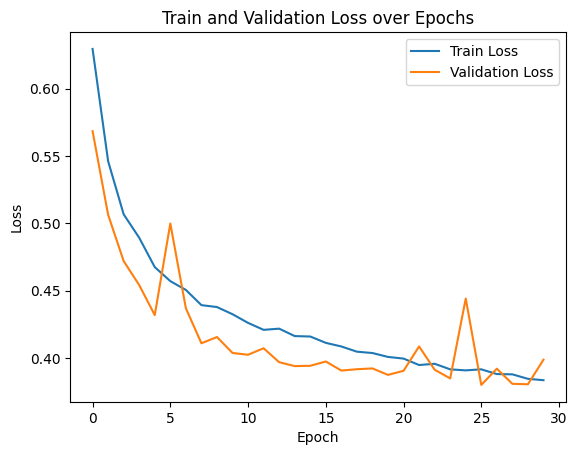
\includegraphics[width=0.50\textwidth]{figure.png}
    \caption{Train and Validation Loss over Epochs}
    \label{fig:Train and Validation Loss over Epochs}
\end{figure}
\newpage



\subsection{(10 Puan)} \textbf{SEED=öğrenci numaranız set ettikten sonra altıncı haftada ödev olarak verdiğim gibi earlystopping'deki en iyi modeli kullanarak, Prensesi İyileştir test setinden accuracy, F1, precision ve recall değerlerini hesaplayan kodu yazın ve sonucu da aşağı yapıştırın. \%80'den fazla başarı bekliyorum test setinden. Daha düşükse başarı oranınız, nerede hata yaptığınızı bulmaya çalışın. \%90'dan fazla başarı almak mümkün (ben denedim).}

\begin{python}
from sklearn.metrics import accuracy_score, precision_score, f1_score, recall_score

def evaluate_metrics(model, criterion, data_loader):
    model.eval()
    y_true = []
    y_pred = []
    losses = []
    
    with torch.no_grad():

        for inputs, labels in data_loader:
            inputs, labels = inputs.to(device), labels.to(device)
            outputs = model(inputs)
            loss = criterion(outputs, labels)
            losses.append(loss.item())
            _, preds = torch.max(outputs, 1)
            y_true.extend(labels.cpu().numpy())
            y_pred.extend(preds.cpu().numpy())
            
    acc = accuracy_score(y_true, y_pred)
    prec = precision_score(y_true, y_pred, average='weighted')
    f1 = f1_score(y_true, y_pred, average='weighted')
    recall = recall_score(y_true, y_pred, average='weighted')
    
    print(f"Test Accuracy: {acc:.4f},Prec Accuracy: {prec:.4f},F1 score: {f1:.4f},Recall score: {recall:.4f}")


evaluate_metrics(model, criterion, validation_loader)
\end{python}

Test Accuracy: 0.9268,Prec Accuracy: 0.9319,F1 score: 0.9266,Recall score: 0.9268
\subsection{(5 Puan)} \textbf{Tüm kodların CPU'da çalışması ne kadar sürüyor hesaplayın. Sonra to device yöntemini kullanarak modeli ve verileri GPU'ya atıp kodu bir de böyle çalıştırın ve ne kadar sürdüğünü hesaplayın. Süreleri aşağıdaki tabloya koyun. GPU için Google Colab ya da Kaggle'ı kullanabilirsiniz, iki ortam da her hafta saatlerce GPU hakkı veriyor.}

\begin{table}[ht!]
    \centering
    \caption{Buraya bir açıklama yazın}
    \begin{tabular}{c|c}
        Ortam & Süre (saniye) \\\hline
        CPU &  0:00:14.163842   \\
        GPU &  0:00:13.492997 \\
    \end{tabular}
    \label{tab:my_table}
\end{table}

\subsection{(3 Puan)} \textbf{Modelin eğitim setine overfit etmesi için elinizden geldiği kadar kodu gereken şekilde değiştirin, validasyon loss'unun açıkça yükselmeye başladığı, training ve validation loss'ları içeren figürü aşağı koyun ve overfit için yaptığınız değişiklikleri aşağı yazın. Overfit, tam bir çanak gibi olmalı ve yükselmeli. Ona göre parametrelerle oynayın.}


Regularization kullanılmadı
Her epochtan sonra val loss değeri kademeli bir şekilde artırıldı.

% Figür aşağı

\begin{figure}[ht!]
    \centering
    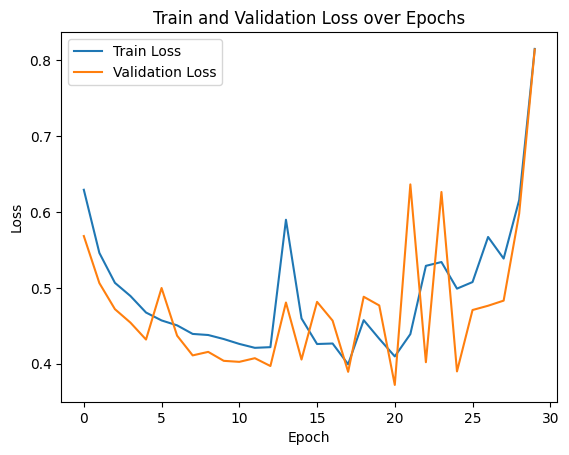
\includegraphics[width=0.75\textwidth]{overfit.png}
    \caption{Overfitting}
    \label{fig:overfitting}
\end{figure}

\newpage

\subsection{(2 Puan)} \textbf{Beşinci soruya ait tüm kodların ve cevapların olduğu jupyter notebook'un Github linkini aşağıdaki url'e koyun.}

\url{https://github.com/haticesaike/neural_network_mid/tree/main/5}

\section{(Toplam 10 Puan)} \textbf{Bir önceki sorudaki Prensesi İyileştir problemindeki yapay sinir ağınıza seçtiğiniz herhangi iki farklı regülarizasyon yöntemi ekleyin ve aşağıdaki soruları cevaplayın.} 

\subsection{(2 puan)} \textbf{Kodlarda regülarizasyon eklediğiniz kısımları aşağı koyun:} 

\begin{python}
def train(model, optimizer, criterion, train_loader, val_loader, num_epochs):

    best_loss = float('inf')
    for epoch in range(num_epochs):
        running_loss = 0.0
        running_corrects = 0
        total_train = 0
        
        model.train() 
        
        for inputs, labels in train_loader:
            inputs, labels = inputs.to(device), labels.to(device)
            optimizer.zero_grad() 
            
            # forward + backward + optimize
            outputs = model(inputs)
            loss = criterion(outputs, labels)
            
            #l2 reg
            # l2_lambda = 0.001
            # l2_reg = torch.tensor(0., device=device)
            # for param in model.parameters():
            #   l2_reg += torch.norm(param)
            # loss += l2_lambda * l2_reg
           
            l1_lambda = 0.001
            l1_reg = torch.tensor(0., requires_grad=False, device=device) 
            for param in model.parameters():
                l1_reg += torch.norm(param, p=1)
            loss += l1_lambda * l1_reg.float() 
            loss.backward()
            optimizer.step()
            
            running_loss += loss.item()
            _, preds = torch.max(outputs, 1)
            running_corrects += torch.sum(preds == labels.data)
            total_train += labels.size(0)
            
        train_loss = running_loss / len(train_loader)
        train_acc =100. * running_corrects / total_train
        train_losses.append(train_loss)
        train_accs.append(train_acc)
        
        
        val_loss, val_acc = evaluate(model, criterion, val_loader)
        val_losses.append(val_loss)
        val_accs.append(val_acc)
        
        
        print(f"Epoch {epoch+1}/{num_epochs} - Train Loss: {train_loss:.4f} - Train Acc: {train_acc:.2f} - Val Loss: {val_loss:.4f} - Val Acc: {val_acc:.2f}")
        
        
        if val_loss < best_loss:
            best_loss = val_loss
            best_model = model.state_dict()
            epochs_no_improve = 0
        else:
            epochs_no_improve += 1
            if epochs_no_improve == 5:
                print("Early stopping!")
                break


def evaluate(model, criterion, data_loader):
    running_loss = 0.0
    running_corrects = 0
    total_val = 0

    model.eval() 

    with torch.no_grad(): 
        for inputs, labels in data_loader:
            inputs, labels = inputs.to(device), labels.to(device)

            outputs = model(inputs.float())
            loss = criterion(outputs, labels)
            #l2 reg
            # l2_lambda = 0.001
            # l2_reg = torch.tensor(0., device=device)
            # for param in model.parameters():
            #   l2_reg += torch.norm(param)
            # loss += l2_lambda * l2_reg
            
            #l1 reg
            l1_lambda = 0.001
            l1_reg = torch.tensor(0., requires_grad=False, device=device) 
            for param in model.parameters():
                l1_reg += torch.norm(param, p=1)
            loss += l1_lambda * l1_reg.float() 
            
            running_loss += loss.item()
            _, preds = torch.max(outputs, 1)
            running_corrects += torch.sum(preds == labels.data)
            total_val += labels.size(0)

    val_loss = running_loss / len(data_loader)
    val_acc = 100. *running_corrects / total_val

    return val_loss, val_acc
train(model, optimizer, criterion, train_loader, validation_loader, num_epochs)

\end{python}

\subsection{(2 puan)} \textbf{Test setinden yeni accuracy, F1, precision ve recall değerlerini hesaplayıp aşağı koyun:}

\newline L1:
Test Accuracy: 0.9204,Prec Accuracy: 0.9267,F1 score: 0.9201,Recall score: 0.9204\newline 

L2:Test Accuracy: 0.9268,Prec Accuracy: 0.9319,F1 score: 0.9266,Recall score: 0.9268\newline 
\newpage

\subsection{(5 puan)} \textbf{Regülarizasyon yöntemi seçimlerinizin sebeplerini ve sonuçlara etkisini yorumlayın:}

L1 ve L2 regülarizasyonu, makine öğrenmesinde aşırı uydurma (overfitting) sorununu çözmek için kullanılan tekniklerdir. Bu teknikler, modelin genellemesini artırarak aşırı uydurmaya neden olan parametreleri sınırlar.

L1 regülarizasyonu, Lasso olarak da bilinir ve parametreleri sıfıra yakınlaştırır. Bu, özellik seçimi yapar ve modeldeki gereksiz özelliklerin ağırlığını sıfıra indirerek daha basit bir model elde edilmesini sağlar.

L2 regülarizasyonu, Ridge olarak da bilinir ve parametreleri küçültür. Bu, parametreleri sıfıra yaklaştırmak yerine küçültür, böylece modelin genellemesi artar ve aşırı uydurma sorunu azalır. Ayrıca, L2 regülarizasyonu, çoklu doğrusal bağlantı (multicollinearity) gibi diğer sorunları da çözer.

L1 ve L2 regülarizasyonu, farklı özelliklere sahip veri kümelerinde farklı sonuçlar verebilir. Genel olarak, L2 regülarizasyonu daha sık kullanılır çünkü daha az agresif olduğu ve daha iyi sonuçlar verdiği düşünülür. Ancak, L1 regülarizasyonu, özellik seçimi için daha uygun olabilir.

Özetle, L1 ve L2 regülarizasyonu, aşırı uydurma sorununu çözmek için kullanılan faydalı tekniklerdir ve hangisinin kullanılacağı veri setinin özelliklerine bağlıdır.

L2 regülarizasyonu, parametreleri daha yumuşak bir şekilde kısıtladığı ve overfitting'e karşı daha iyi koruma sağladığı için daha iyi sonuç verdi.

\subsection{(1 puan)} \textbf{Sonucun github linkini  aşağıya koyun:}

\url{https://github.com/haticesaike/neural_network_mid/blob/main/6/MLP_Regularization.ipynb}

\end{document}